\documentclass[12pt]{article}
\usepackage[numbers]{natbib}
\usepackage{amsmath}
\usepackage{hyperref}
\usepackage[a4paper, margin=1in]{geometry}
\usepackage{subcaption}
\usepackage{float}


% === Language and Fonts ===
\usepackage[english]{babel}  % Set document language
\usepackage[utf8]{inputenc}  % Input encoding
\usepackage[T1]{fontenc}  % Font encoding for better hyphenation
\usepackage{times}  % Use Times New Roman font (optional)

% === Graphics and Figures ===
\usepackage{graphicx}  % Include images
\usepackage{caption}  % Enhance captions
\captionsetup{font=small, labelfont=bf}

% === Header and Footer ===
\usepackage{fancyhdr}
\fancyhf{}  % Clear default settings
\fancyhead[L]{\nouppercase{\leftmark}}  % Display chapter title in header
\fancyfoot[C]{\thepage}  % Page number in footer
\pagestyle{fancy}

% === Hyperlinks ===
\usepackage{hyperref}  % Enable clickable links
\hypersetup{
    colorlinks=true,
    linkcolor=blue,
    citecolor=blue,
    urlcolor=blue,
    pdftitle={Subsurface Features of Lunar Pits},
    pdfauthor={Michal Glos}
}


\begin{document}

\begin{titlepage}
    \centering
    \vspace{3cm}
    \includegraphics[width=0.22\textwidth]{img/fekt-logo.png} \\
    \vspace{0.5cm}
    
    {\scshape\large\bfseries Brno University of Technology \par}
    {\scshape\normalsize Faculty of Electrical Engineering \\ and Communication \par}
    \vspace{3.33cm}
    
    {\Huge\bfseries Subsurface Features of Lunar Pits} \\ 
    {\Large\bfseries\vspace{0.5cm} A Contemporary Survey \par}
    \vspace{2.66cm}

    {\LARGE\bfseries Team Project (TEP)} \\
    {\Large Space Applications\par}
    \vspace{3.33cm}
    
    {\Large by \par}
    {\Large\bfseries Michal Glos (213396) \par}
    \vfill

    
    {\large December 2024 \par}
\end{titlepage}


\begin{abstract}
Lunar pits, discovered through high-resolution imagery from missions such as the Lunar Reconnaissance Orbiter (LRO) and SELENE, are transformative geological features that provide unparalleled access to the Moon's subsurface. These pits reveal ancient stratigraphic layers, offering insights into volcanic processes and the evolution of the lunar crust. Beyond their geological significance, they present practical opportunities as stable, sheltered environments that could support future exploration, habitation, and resource utilization. This work consolidates current understanding of lunar pit morphology, formation mechanisms, thermal properties, and spatial distribution, integrating key findings from radar imaging, thermal modeling, and gravitational studies. With their potential to serve as gateways to subsurface voids and natural laboratories for planetary science, lunar pits are emerging as critical focal points in the pursuit of sustainable lunar exploration and habitation strategies.
\end{abstract}


\graphicspath{{img/ch1}}

\section{Introduction}
Lunar pits are remarkable geological formations that differ significantly from impact craters and volcanic vents. Characterized by steep vertical walls, these features often provide direct access to subsurface voids, such as collapsed lava tubes, tectonic cavities, or impact-induced hollows \cite{lunar-pit-distribution, lunar-pits-entrances-to-caves, new-wagner}. Their discovery, largely enabled by high-resolution imagery from the Lunar Reconnaissance Orbiter (LRO) Narrow Angle Camera (NAC) and the SELENE spacecraft, has revolutionized our understanding of the Moon's crustal architecture, composition, and dynamic history. For example, GRAIL and SELENE data reveal gravity anomalies and radar echoes consistent with intact lava tubes beneath some pits, such as the Marius Hills region \cite{GRAIL, cavities-selene-lavatubes, grails-gradients-mariushills}.

Beyond their geological intrigue, lunar pits hold practical importance for future exploration. These natural formations offer stable thermal environments, shielding from cosmic radiation, and protection from micrometeoroid impacts, making them attractive candidates for human habitation, resource storage, and scientific research stations \cite{bases-feng, newer-thermal, radar-observations-lava-tubes}. Notably, the Mare Tranquillitatis pit (see Fig.~\ref{fig:image1}), a vertical shaft with visible stratigraphic layers, exemplifies the potential of such features to provide insights into lunar geology and serve as access points to extensive cave systems. Radar imaging has further confirmed a subsurface cave conduit beneath the Mare Tranquillitatis pit, supporting its suitability as a target for human exploration \cite{Carrer2024, grails-gradients-mariushills}.

Lunar pits expose ancient stratigraphic layers, revealing records of volcanic flows and crustal evolution. Observations from missions such as SELENE and LRO confirm that these features likely formed through roof collapses above voids, such as lava tubes, highlighting their volcanic origin. For example, the Mare Tranquillitatis pit has been modeled to result from impacts triggering collapses in lava tube roofs, a process corroborated by gravitational anomalies and radar data \cite{lunar-pits-numerical-modelling, radar-observations-lava-tubes, cavities-selene-lavatubes}. The internal layering visible in pits, such as those in Mare Tranquillitatis and Marius Hills, provides key data on successive volcanic episodes, supporting broader studies on lunar surface evolution \cite{sublunear-lava, newer-thermal, bases-feng}.

\begin{figure}[h!]
    \centering
    \begin{subfigure}[c]{0.59\linewidth}
        \centering
        \includegraphics[width=0.9\linewidth]{lunar-pits-with-layers.png}
        \caption{Close-up images of the Mare Tranquillitatis pit, showcasing visible stratigraphic layers (segmentation in Figure \textbf{F}). Images A and B reveal over 90 \% of the pit floor using \textbf{LRO NAC} data. Figure adapted from \cite{sublunear-lava}.}
        \label{fig:image1}
    \end{subfigure}
    \hfill
    \begin{subfigure}[c]{0.4\linewidth}
        \centering
        \includegraphics[width=0.9\linewidth]{Lunar_Pit_layers_2pic_location.png}
        \caption{Location of the Mare Tranquillitatis pit, captured by \textbf{LRO WAC}. Figure adapted from \cite{sublunear-lava}.}
        \label{fig:image2}
    \end{subfigure}
\end{figure}

\subsection{Discovery and Recognition}
The identification of lunar pits was delayed until the advent of advanced lunar missions, as these features are relatively small and difficult to observe using Earth-based telescopes \cite{lunar-pit-distribution}. Early evidence emerged from SELENE and LRO data, which revealed steep-walled pits with distinct overhangs and evidence of hollow subsurface structures. For instance, the Mare Tranquillitatis pit has been confirmed to connect to a subsurface void, tens of meters long, using radar and gravitational techniques, transforming pits from geological curiosities to priority targets for lunar exploration \cite{Carrer2024, GRAIL, radar-observations-lava-tubes}.

The Mare Tranquillitatis pit, in particular, has been the focus of radar and imaging studies that confirmed its connection to a subsurface cave conduit. These findings not only demonstrate the scientific value of pits for studying lunar geology but also highlight their potential for human exploration. Advanced thermal modeling, such as that performed using Diviner data, shows that the interior of pits remains thermally stable compared to the extreme surface environment, reinforcing their suitability as habitats or resource storage sites \cite{newer-thermal, lunar-pits-entrances-to-caves, thermal-lunar-pits}.

As technology advances, the exploration of lunar pits continues to evolve. With 3D thermal models, radar imaging, and gravitational studies, these features are increasingly seen as critical to understanding the Moon’s history and unlocking future possibilities for sustained human presence on its surface \cite{newer-thermal, radar-observations-lava-tubes, grails-gradients-mariushills}.

\newpage

\graphicspath{{img/ch2}}

\section{Lunar Pit Geological Characteristics}

\subsection{Morphological Characteristics}

Lunar pits exhibit distinct morphological features that provide critical insights into their geological origins and evolution. Typically characterized by funnel-shaped upper regions leading into near-vertical walls, these pits often terminate in flat or slightly concave floors \cite{new-wagner, lunar-pits-numerical-modelling, lunar-pit-distribution}. The sharp transition between the sloping entrance and vertical walls suggests that these features form primarily due to sudden roof collapses above subsurface voids, rather than gradual erosion processes \cite{lunar-pits-numerical-modelling, new-wagner}.

\begin{figure}[h!]
    \centering
    \includegraphics[width=0.5\linewidth]{lunar_pit_schema.png}
    \caption{A simplified schematic of a generic lunar pit cross-section showing key morphological features (adapted from \cite{new-wagner}).}
    \label{fig:lunar-pit-schema}
\end{figure}

High-resolution images from the Lunar Reconnaissance Orbiter (LRO) Narrow Angle Camera (NAC) have revealed significant details, such as stratified layering within pit walls, which likely correspond to successive volcanic flow events. These layers provide critical geological records of ancient lunar volcanism \cite{lunar-pits-entrances-to-caves, Carrer2024}. Overhangs within pits, such as those in Mare Tranquillitatis and Marius Hills, indicate access to extensive subsurface voids consistent with collapsed lava tubes. These voids could extend tens of meters and present exciting opportunities for future robotic exploration missions \cite{lunar-pits-numerical-modelling, radar-observations-lava-tubes}.

The bases of lunar pits commonly accumulate boulders and regolith, which can obscure deeper portions of the pits and affect depth measurements. Concave floors can alter the perceived depth by visually increasing the vertical extent of the pit's interior relative to its surroundings \cite{lunar-pit-distribution, new-wagner}. This contrasts with traditional impact craters, which are characterized by raised rims and ejecta blankets.

Over geological timescales, lunar pits degrade due to micrometeoroid impacts, thermal cycling, and seismic activity. These processes erode walls and rims, depositing debris at the base. Mare Tranquillitatis, which retains sharp walls and minimal infill, contrasts with Marius Hills pits, where smoother, partially infilled floors indicate older, more degraded structures. This variation in preservation demonstrates the gradual evolution of lunar pits over hundreds of millions of years, largely independent of surrounding terrain age \cite{lunar-pit-distribution, radar-observations-lava-tubes, newer-thermal}.

\begin{figure}[H]
    \centering
    \includegraphics[width=0.85\linewidth]{closed_and_open_cavities.png}
    \caption{Progression of lunar pit degradation, illustrating gradual erosion and regolith deposition over time. The figure shows different lunar pits in various stages of erosion (adapted from \cite{new-wagner}).}
    \label{fig:lunar-pit-degradation}
\end{figure}

\subsection{Geographical Distribution and Formation Mechanisms}

Lunar pits are distributed across three primary geological settings: mare basalts, impact melt deposits, and highland terrain. Each setting reflects distinct formation mechanisms and geological implications \cite{lunar-pit-distribution, radar-observations-lava-tubes}.

\begin{figure}[H]
    \centering
    \includegraphics[width=0.98\linewidth]{map-lunar-pits-rough.png}
    \caption{Map of lunar pits: eight in mare basalts, two in highlands (stars), and 29 in impact melt deposits (dots). Figure adapted from \cite{lunar-pit-distribution}. This map is from 2014, currently, more then 300 lunar pits were discovered.}
    \label{fig:map-lunar-pits}
\end{figure}

\paragraph{Mare Basalts}
Pits in mare regions, such as Marius Hills and Mare Tranquillitatis, are predominantly linked to volcanic activity. These pits are hypothesized to form through the collapse of lava tube roofs, as overlying material becomes unstable and collapses into voids below \cite{lunar-pits-entrances-to-caves, radar-observations-lava-tubes}. Radar and imaging data from Mare Tranquillitatis reveal extensive subsurface voids consistent with intact lava tubes, which serve as potential habitats or scientific exploration targets \cite{Carrer2024, radar-observations-lava-tubes}.

\begin{figure}[H]
    \centering
    \includegraphics[width=0.7\linewidth]{lava_tube_formation_schema.png}
    \caption{Stages of lunar lava tube formation, illustrating crust solidification, lava drainage, and resulting voids (adapted from \cite{lunar-pits-entrances-to-caves}).}
    \label{fig:lava-tube-formation-schema}
\end{figure}

\paragraph{Impact Melt Deposits}
Pits found within impact craters, such as Tycho and Copernicus, form due to high-energy impacts that fracture and compress the lunar crust, generating molten material. As this molten material cools, thermal contraction creates cracks and fractures that eventually collapse into pits. These features are typically circular in shape, lack overhangs, and have no association with lava flows \cite{clrn-impact-melt, lunar-pits-numerical-modelling}.

\begin{figure}[H]
    \centering
    \includegraphics[width=0.42\linewidth]{Impact-Shock-Pressures-and-Their-Effects-1024x857.jpg}
    \caption{Impact dynamics illustrating pressure zones, molten material, and the formation of cracks contributing to pit formation in impact melt deposits (adapted from \cite{clrn-impact-melt}).}
    \label{fig:impact-melt}
\end{figure}

\paragraph{Highland Terrain}
Highland pits, such as those in Lacus Mortis, are thought to result from tectonic stresses and extensional faulting. These pits typically form near graben systems or faulted regions, where crustal stress generates fractures. Over time, localized collapses along these fault zones create pits with sharp, near-vertical walls. Unlike mare pits, highland pits lack volcanic associations, emphasizing their tectonic origin \cite{new-wagner, lunar-pit-distribution}. 

While mare pits are often associated with extensive sublunarean cavities, highland pits generally lack direct evidence of such voids. Their formation mechanisms, primarily driven by tectonic activity, may result in smaller or less interconnected voids compared to those formed by lava tube collapses. Current studies, such as those by Wagner et al. (2022), have not confirmed large, accessible sublunarean cavities within highland terrain pits, limiting their potential for exploration of extensive underground structures \cite{lunar-pit-distribution, radar-observations-lava-tubes, cavities-selene-lavatubes}.

\begin{figure}[H]
    \centering
    \includegraphics[width=0.33\linewidth]{lunar-pit-highland.png}
    \caption{Lunar Reconnaissance Orbiter Camera footage of Lacus Mortis Pit. Image adapted from: \url{https://www.lroc.asu.edu/atlases/pits}.}
    \label{fig:highland-lunar-pit}
\end{figure}

\paragraph{Impact-Induced Skylights}
Unlike the formation mechanisms described above, impact-induced skylights are not a primary formation mechanism but occur when small meteoroid impacts destabilize thin crusts overlying intact voids, such as lava tubes. Numerical simulations suggest that impacts create localized collapses, such as the 26-meter-thick roof collapse in Marius Hills, forming a skylight approximately 40 meters wide. These simulations highlight skylights as secondary features of great interest for exploration \cite{clrn-impact-melt, lunar-pits-numerical-modelling}.

\begin{figure}[H]
    \centering
    \includegraphics[width=0.99\linewidth]{lunar-pit-in-lava-tube.png}
    \caption{Cross section of a lunar tube with collapsed skylight (adapted from \cite{bases-feng}).}
    \label{fig:impact-induced-skylight}
\end{figure}




\graphicspath{{img/ch3}}

\section{Thermal Characteristics}

\subsection{Thermal Stability and Anomalies}

The thermal environment within lunar pits provides a stark contrast to the extreme temperature fluctuations of the lunar surface. Data collected from the Diviner Lunar Radiometer Experiment reveal that the interior of pits maintains remarkably stable temperatures, with values ranging from approximately 250 to 290 K in permanently shadowed regions, even during the lunar night \cite{thermal-lunar-pits}. This is in contrast to the lunar surface, where temperatures vary dramatically between $\sim$100 K during the night and $\sim$400 K in direct sunlight due to the Moon’s lack of atmosphere.

\begin{figure}[H]
    \centering
    \includegraphics[width=0.6\linewidth]{lunar-pit-thermal-model.png}
    \caption{Schematic representation of heat transfer in lunar pits, illustrating shadowing, infrared emission, and subsurface conduction \cite{thermal-lunar-pits}.}
    \label{fig:lunar-pit-thermal-model}
\end{figure}

The thermal stability observed in pits results primarily from their geometry. Overhanging walls and limited sky exposure block direct solar radiation and mitigate radiative heat loss during the lunar night. As modeled by Horvath et al. \cite{thermal-lunar-pits}, this creates natural “blackbody cavities,” where incoming solar radiation is absorbed and redistributed internally. The floors of pits, such as those in Mare Tranquillitatis and Mare Ingenii, have been observed to remain up to 100 K warmer than the surrounding surface at night, confirming their thermal insulating properties \cite{thermal-lunar-pits, newer-thermal}.

\begin{figure}[H]
    \centering
    \includegraphics[width=0.7\linewidth]{lunar-pits-temperature-LROC.png}
    \caption{Temperature maps of Mare Tranquillitatis (a) and Mare Ingenii pits (b) measured by Diviner. Insets show NAC images for reference. Warm anomalies appear in pit interiors compared to surrounding surfaces \cite{thermal-lunar-pits}.}
    \label{fig:lunar-pits-temperatures-LROC}
\end{figure}

\subsection{Thermal Dynamics and Material Effects}

The thermal behavior of pit floors and walls is strongly influenced by their material composition. Numerical models comparing regolith-dominated and rock-dominated surfaces reveal key differences in diurnal temperature variations. Rock surfaces exhibit smaller temperature fluctuations due to their higher thermal conductivity, which allows for more efficient heat transfer and rapid equilibration. In contrast, regolith-covered surfaces show larger diurnal variations, as the insulating properties of lunar soil slow heat exchange, leading to higher daytime peaks and lower nighttime minima \cite{thermal-lunar-pits, newer-thermal}.

\begin{figure}[H]
    \centering
    \includegraphics[width=0.9\linewidth]{lunar-pit-regolith-vs-stone-thermal.png}
    \caption{Simulated temperature profiles for lunar pits assuming regolith (c) and solid rock (d) floors. Rock surfaces show smaller diurnal variations due to higher thermal conductivity, while regolith exhibits greater fluctuations \cite{thermal-lunar-pits}.}
    \label{fig:regolith-vs-stone-thermal}
\end{figure}

This behavior has important implications for thermal stability. Pits with rocky floors maintain temperatures closer to equilibrium values due to their ability to distribute absorbed heat efficiently. Conversely, regolith-covered floors experience more pronounced temperature extremes, as their insulating nature restricts heat dissipation. These findings provide insights into the expected thermal environment within pits and can guide the selection of potential exploration and habitation sites.

\begin{figure}[H]
    \centering
    \includegraphics[width=0.75\linewidth]{thermal-simulation-lunar-pits-2d-regolith-rock.png}
    \caption{Equilibrium temperature distributions for rock (a, c) and regolith (b, d) surfaces in lunar pits and caves. The top row shows extended horizontal caves, while the bottom row focuses on vertical pits. Regolith surfaces (b, d) retain heat closer to the opening, while rock surfaces (a, c) exhibit cooler and more uniform internal temperatures \cite{thermal-lunar-pits}.}
    \label{fig:lunar-pit-equilibrium-temps}
\end{figure}


\subsection{Volatile Stability and Cold Traps}

Lunar pits have also been proposed as potential cold traps for volatiles, such as water ice, particularly in high-latitude regions. However, recent studies indicate that the enclosed geometry of pits leads to multiple scattering of infrared radiation, which raises internal temperatures and reduces their efficiency as cold traps compared to traditional craters \cite{newer-thermal}. Nevertheless, specific conditions—such as pits shadowed by exterior topography or connected to deeper caves—may still support the accumulation of volatiles \cite{newer-thermal, lunar-pits-numerical-modelling}.

Wilcoski et al. \cite{newer-thermal} demonstrate that volatile loss rates within pits are generally higher than in permanently shadowed regions (PSRs) of craters, making pits less efficient for long-term ice storage. However, their potential to provide protection from surface processes, such as micrometeoroid impacts and solar wind sputtering, remains an advantage for short-term volatile preservation.


\graphicspath{{img/ch4}}

\section{Evidence of Cavities Beneath Lunar Pits}

Evidence for subsurface cavities beneath lunar pits is derived from morphological observations, geophysical gravity anomalies, radar sounder reflections, and thermal data. These findings point to large, interconnected voids beneath regions such as \textbf{Marius Hills} and \textbf{Mare Tranquillitatis}, supporting their interpretation as remnants of ancient lava tubes and key features of lunar geological evolution.

\subsection{Morphological Evidence}

Overhanging walls and roof collapses in lunar pits strongly suggest access points to larger subsurface voids, such as intact lava tubes (see Fig. \ref{fig:image1}). High-resolution imagery from the Lunar Reconnaissance Orbiter (LROC) has revealed alignments between these pits and sinuous rilles—ancient lava flow channels associated with underground tubes \citep{lunar-pits-entrances-to-caves, grails-gradients-mariushills}. The Marius Hills region, in particular, shows clear morphological correlations with known volcanic features, as seen in Figure~\ref{fig:marius-hills-collapse}.

\textbf{Collapse Chains and Pit Alignments:} Linear sequences of pits, known as collapse chains, further support the hypothesis of underlying cavities. These chains represent the progressive collapse of lava tube roofs, forming surface depressions that trace the subsurface voids. This is particularly evident in Marius Hills, where pit alignments correlate with surface rilles and lava tubes observed on Earth \citep{new-wagner, cavities-selene-lavatubes}.

\begin{figure}[H]
    \centering
    \includegraphics[width=0.5\linewidth]{marius_hills_collapse.png}
    \caption{LROC WAC image of the Marius Hills region, showing collapse chains, sinuous rilles, and skylights. The red dashed line marks the approximate path of the subsurface lava tube. 
    \textbf{(a)} Overview of the Marius Hills region with localized collapse chains and skylights. 
    \textbf{(b)} Close-up of the Marius Hills Hole (MHH). 
    \textbf{(c)} Marius-B collapse chain. 
    \textbf{(d)} Marius-A collapse chain. 
    Adapted from \citet{grails-gradients-mariushills}.}
    \label{fig:marius-hills-collapse}
\end{figure}

\subsection{Geophysical Evidence}

\textbf{Gravity Anomalies from GRAIL:} Subsurface cavities induce detectable gravitational anomalies due to mass deficits in hollow regions. Data from the \textbf{Gravity Recovery and Interior Laboratory (GRAIL)} mission has revealed mass deficits beneath several pit locations. For example, in Marius Hills, Bouguer gravity gradients identified a hollow structure approximately 60 km long and 9 km wide at a depth of 600 m \citep{grails-gradients-mariushills}. These anomalies align closely with pit locations and other volcanic features.

\begin{figure}[H]
    \centering
    \includegraphics[width=0.85\linewidth]{grail-images-grabity.png}
    \caption{Gravitational anomalies in the Marius Hills region detected by GRAIL. Bouguer gravity gradients reveal mass deficits (blue), indicative of subsurface voids such as intact lava tubes. Adapted from \citet{grails-gradients-mariushills}.}
    \label{fig:marius-hills-gravity}
\end{figure}

\subsection{Radar Evidence from SELENE and Mini-RF}

\textbf{Radar Echoes from SELENE (Kaguya):} Radar sounders like the Lunar Radar Sounder (LRS) onboard SELENE have been instrumental in confirming subsurface cavities. Double-echo patterns—secondary radar reflections—indicate voids beneath the lunar surface. At Mare Tranquillitatis, LRS data suggest a subsurface cavity extending several kilometers \citep{cavities-selene-lavatubes}.

\begin{figure}[H]
    \centering
    \includegraphics[width=0.35\linewidth]{selene-doublebump.png}
    \caption{SELENE LRS radar echoes showing a characteristic double-echo pattern indicative of a subsurface void. The first peak represents the surface reflection, while the second peak corresponds to the void floor. Adapted from \citep{cavities-selene-lavatubes}.}
    \label{fig:radar-echoes}
\end{figure}

\textbf{Mini-RF Contributions:} Using Mini-RF data, Carrer et al. (2024) identified radar reflections beyond the walls of Mare Tranquillitatis Pit. These reflections are consistent with a lava tube connected to the pit. Combined with gravitational and morphological data, this strengthens the hypothesis of intact subsurface voids \citep{Carrer2024}.

\begin{figure}[H]
    \centering
    \includegraphics[width=0.85\linewidth]{carrer-renders.png}
    \caption{Reconstructed Mare Tranquillitatis Pit (MTP) cave conduit based on inversion of Mini-RF radar data. \textbf{(a)} Model A with a conduit of approximately 135 m width and a low floor slope. \textbf{(b)} Model B with a conduit approximately 175 m wide and steeper floor slopes. The 3D models show the surface (yellow), subsurface lava flows (blue), and inferred lava tube conduit (gray). Adapted from \citep{Carrer2024}.}
    \label{fig:mtp-cave-conduit}
\end{figure}

\subsection{Thermal Observations as Indirect Evidence}

Thermal data also suggest subsurface cavities beneath pits. The Diviner Lunar Radiometer Experiment has shown that the interiors of pits maintain stable temperatures, supporting the idea of thermally buffered environments consistent with underground voids. For example, temperatures within the Mare Tranquillitatis pit remain near -25°C throughout the lunar night, suggesting limited thermal exposure due to cavity geometry \citep{thermal-lunar-pits, newer-thermal}.

This stability aligns with the blackbody cavity effect, where limited exposure to sunlight and the insulating properties of surrounding rock create stable conditions. Such environments could provide ideal conditions for exploration and resource utilization.

\graphicspath{{img/ch5}}
\section{Related Unmanned Missions}

The exploration of lunar pits and lava tubes has transitioned from observational curiosities to key objectives in planetary science and lunar exploration. These missions provide essential insights into the Moon’s volcanic history and potential access to subsurface voids.

\subsection{Past Missions}

\textbf{Apollo Program:}  
The Apollo program laid the foundation for modern lunar exploration by providing essential geological and subsurface data. Apollo 15 identified Hadley Rille, a collapsed lava tube, while Apollo 17’s Apollo Lunar Sounder Experiment (ALSE) utilized radar to detect subsurface voids and structural discontinuities, suggesting the presence of lava tubes and faults beneath the surface. ALSE's pioneering radar observations demonstrated the potential of subsurface mapping on the Moon and influenced the design of future missions, such as SELENE and Chang’e \cite{radar-observations-lava-tubes}.

\textbf{SELENE (Kaguya):}  
Japan's SELENE (Kaguya) mission, launched in 2007, provided groundbreaking evidence of intact lava tubes using the Lunar Radar Sounder (LRS). Double-echo radar patterns near the Marius Hills Hole (MHH) confirmed the existence of hollow subsurface structures, with void dimensions and roof thickness inferred from radar analysis. These findings offered unprecedented insights into lunar volcanic history and the stability of subsurface cavities. SELENE’s high-resolution imagery further complemented radar data, enabling detailed mapping of the lunar surface and its volcanic features \cite{cavities-selene-lavatubes, radar-observations-lava-tubes}.

\textbf{Chang’e Missions (China):}  
China’s Chang’e program advanced subsurface exploration through ground-penetrating radar (GPR) deployed on Chang’e-3 and Chang’e-4. These missions mapped regolith layers and detected subsurface voids, with Chang’e-4 providing unique data from the lunar far side. High-resolution radar from these missions revealed stratified geological layers and potential lava tube structures beneath the regolith, enhancing understanding of lunar geology and informing future mission planning \cite{radar-observations-lava-tubes, cavities-selene-lavatubes}.

\subsection{Active Missions}

\textbf{Lunar Reconnaissance Orbiter (LRO):}  
NASA’s LRO has played a pivotal role in mapping lunar pits and identifying their connections to subsurface features:
\begin{itemize}
    \item The \textbf{Narrow Angle Camera (NAC)} discovered over 300 pits, including the well-studied Mare Tranquillitatis pit \cite{thermal-lunar-pits}.
    \item The \textbf{Mini-RF radar} validated links between pits and lava tubes, emphasizing their significance for future exploration \cite{new-wagner}.
    \item The \textbf{Diviner Lunar Radiometer Experiment (DLRE)} revealed thermally stable environments within pits, highlighting their suitability for exploration and habitation \cite{thermal-lunar-pits}.
\end{itemize}

\begin{figure}[h!]
    \centering
    \begin{minipage}{0.48\textwidth}
        \centering
        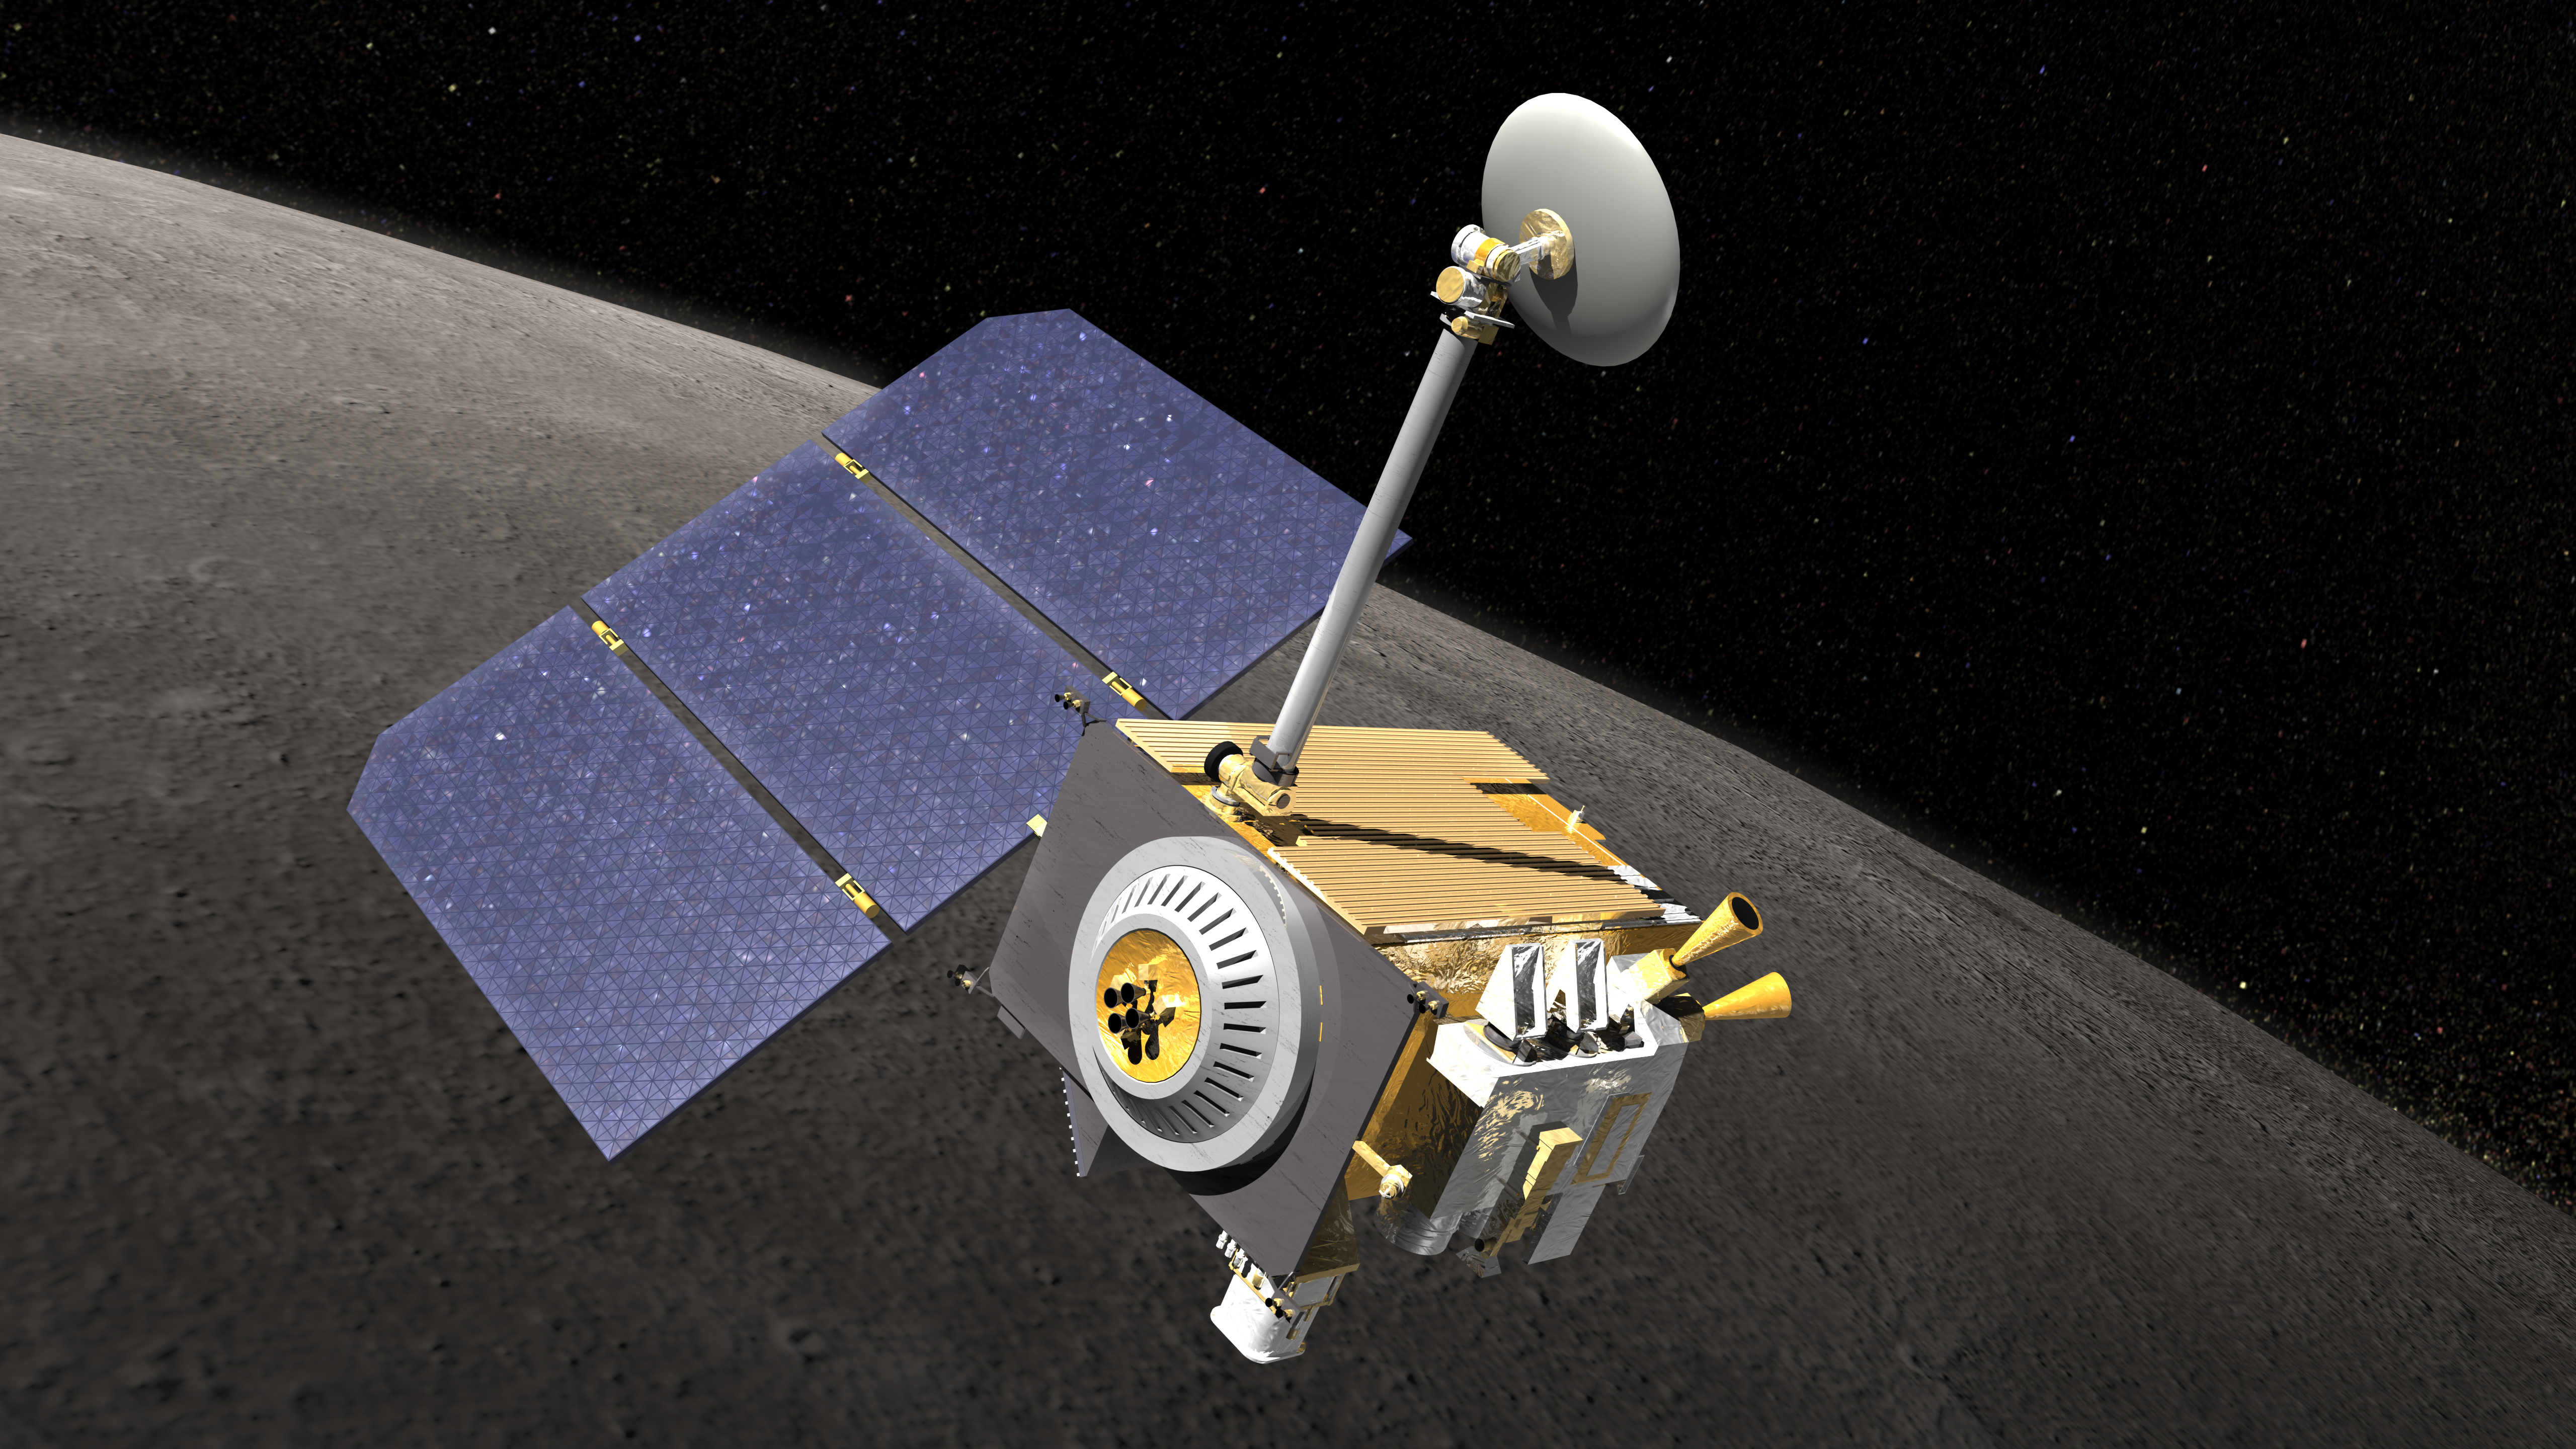
\includegraphics[width=\textwidth]{LROC-render.png}
        \caption{Artistic rendering of the Lunar Reconnaissance Orbiter (LRO) in lunar orbit, adapted from \cite{lro}}
        \label{fig:lro_render}
    \end{minipage}
    \hfill
    \begin{minipage}{0.48\textwidth}
        \centering
        \includegraphics[width=\textwidth]{LROC-schema.png}
        \caption{Schematic of LRO with labeled instruments, adapted from \cite{lro}.}
        \label{fig:lro_schema}
    \end{minipage}
\end{figure}

\textbf{GRAIL (NASA):}  
The Gravity Recovery and Interior Laboratory (GRAIL) mission utilized twin spacecraft, Ebb and Flow, to map the Moon's gravity field with unprecedented precision. Data from GRAIL revealed significant mass deficits beneath the Marius Hills region, strongly indicating the presence of extensive hollow structures, such as lava tubes, that could span up to 60 km in length \cite{grails-gradients-mariushills}.

\begin{figure}[H]
    \centering
    \includegraphics[width=0.52\linewidth]{grail.png}
    \caption{The GRAIL mission satellites used to measure the Moon’s gravity gradients \cite{GRAIL}.}
    \label{fig:grail-render}
\end{figure}

\subsection{Future Planned Missions}

\textbf{Daedalus Rover (ESA):}  
The European Space Agency’s (ESA) Daedalus (Descent And Exploration in Deep Autonomy of Lunar Underground Structures) rover is an advanced mission concept designed to explore the Marius Hills Pit. This skylight provides access to one of the Moon's most prominent lava tubes, making it an ideal candidate for investigating subsurface environments. The Daedalus mission seeks to autonomously map and analyze these environments \cite{esa-daedalus}.

The Daedalus rover is deployed via a tethered descent system to ensure precise placement and communication with the surface. Equipped with advanced 3D lidar and stereo cameras, the rover maps pit interiors and surrounding structures in high resolution, while also analyzing environmental conditions such as structural integrity, radiation, and thermal stability to assess habitability \cite{esa-daedalus}.

A unique feature of Daedalus is its swarm of kinetic energy-based jumping mechanism, which allows it to traverse rugged and uneven terrain. This capability enables it to navigate obstacles and confined spaces that are inaccessible to traditional rovers, making it ideal for exploring lava tubes and subsurface voids. Each jump is carefully controlled for stability and precision upon landing.

\begin{figure}[H]
    \centering
    \includegraphics[width=0.66\linewidth]{daedalus-schema.png}
    \caption{Conceptual diagram of the Daedalus rover’s exploration system, showcasing its tethered deployment and instrumentation \cite{esa-daedalus}.}
    \label{fig:daedalus-mission-schema}
\end{figure}

The jumping mechanism is illustrated below, showing its ability to adapt to challenging environments:

\begin{figure}[H]
    \centering
    \begin{minipage}[b]{0.2\textwidth}
        \centering
        \includegraphics[width=0.5\textwidth]{daedalus-jumper-1.png}
        \caption*{Static position}
    \end{minipage}
    \hspace{0.02\textwidth}
    \begin{minipage}[b]{0.2\textwidth}
        \centering
        \includegraphics[width=0.5\textwidth]{daedalus-jumper-2.png}
        \caption*{Preparing for a jump}
    \end{minipage}
    \hspace{0.02\textwidth}
    \begin{minipage}[b]{0.2\textwidth}
        \centering
        \includegraphics[width=0.5\textwidth]{daedalus-jumper-3.png}
        \caption*{Mid-air jump}
    \end{minipage}
    \caption{Stages of motion for the Daedalus jumping robot, highlighting its innovative locomotion system \cite{esa-daedalus}.}
    \label{fig:lunar_robot_movement}
\end{figure}

\textbf{Moon Diver Mission (NASA):}  
The Moon Diver mission, proposed by NASA, aims to deploy the Axel Extreme Terrain Rover into the Mare Tranquillitatis pit, a 125-meter-deep lunar mare pit with exposed basalt layers. This mission is designed to investigate the geological history and volcanic processes that shaped the Moon, with a particular focus on stratified lava flows visible within the pit walls \cite{kerber2023, nesnas2019}.

The Axel rover is a tethered robotic system uniquely engineered for extreme terrain exploration. Its innovative design includes:
\begin{itemize}
    \item \textbf{Tethered Descent System:} The rover is equipped with a 300-meter tether that provides both mechanical support and power, enabling controlled descent into steep-walled craters while maintaining uninterrupted communication with the lander \cite{kerber2016}.
    \item \textbf{Modular Mobility:} The rover’s dual-wheel configuration and detachable tether arm allow it to maneuver efficiently on uneven surfaces, ensuring adaptability in challenging lunar environments.
    \item \textbf{Scientific Payload:} The rover carries instruments such as the Multispectral Microimager (MMI) for high-resolution imaging of mineralogical features, an Alpha Particle X-ray Spectrometer (APXS) for elemental analysis, and FarCam and CloseCam cameras to document pit stratigraphy and generate 3D topographic models \cite{kerber2023}.
\end{itemize}


\begin{figure}[H]
    \centering
    \begin{minipage}[b]{0.49\textwidth}
        \centering
        \includegraphics[width=\textwidth]{moon-diver-pit-recon.png}
        \caption{3D reconstruction of a terrestrial pit using the Moon Diver prototype. This model demonstrates the rover’s capability to map pit stratigraphy with precision \cite{kerber2023}.}
        \label{fig:moon_diver_3d_recon}
    \end{minipage}
    \hfill
    \begin{minipage}[b]{0.49\textwidth}
        \centering
        \includegraphics[width=\textwidth]{moon-diver-schemoid.png}
        \caption{Schematic visualization of the Axel Rover’s tethered descent system, highlighting its mechanical and power supply features \cite{nesnas2019}.}
        \label{fig:moon_diver_schematic}
    \end{minipage}
\end{figure}

\subsection{Scientific Value of Lunar Pits and Lava Tubes}

Lunar pits and lava tubes provide exceptional opportunities for scientific research, offering unique insights into planetary geology, volcanism, and the Moon's evolutionary history.

\textbf{Preservation of Geological History:}  
The interiors of lava tubes and pits serve as natural archives of the Moon's volcanic activity. Their stable, unaltered environments protect geological features and stratigraphic layers, offering detailed records of past eruptions, lava flow dynamics, and crustal evolution \cite{thermal-lunar-pits, cavities-selene-lavatubes}.

\textbf{Understanding Lunar Volcanism:}  
The exposed layers within pits like the Mare Tranquillitatis provide access to stratified basalt flows, enabling detailed investigations of volcanic processes. These studies help to reconstruct the Moon’s thermal history and assess its geological diversity \cite{kerber2023, grails-gradients-mariushills}.

\textbf{Exploration of Subsurface Voids:}  
Subsurface cavities, identified through radar and gravity anomalies, allow researchers to study the structural integrity and formation mechanisms of large-scale lava tubes. These features highlight differences between terrestrial and lunar volcanism, particularly in terms of scale and stability, attributed to the Moon’s low gravity and lack of atmospheric erosion \cite{cavities-selene-lavatubes, grails-gradients-mariushills}.

\textbf{Astrobiological Potential:}  
The stable thermal environments and potential for volatile accumulation within pits make them analogous to habitable conditions on other celestial bodies. These studies inform astrobiological exploration and guide the search for life-supporting environments beyond Earth \cite{newer-thermal, sublunear-lava}.

\textbf{Comparative Planetology:}  
Lunar pits and lava tubes act as analogs for subsurface voids on other planets, such as Mars. The study of these features enhances our understanding of planetary processes and provides a framework for exploring similar structures on extraterrestrial surfaces \cite{cavities-selene-lavatubes, kerber2016}.


\graphicspath{{img/ch6}}

\section{Potential for Permanent Human Presence}

\subsection{Natural Advantages of Lunar Pits}

\subsubsection{Radiation and Micrometeoroid Shielding}

Lunar pits provide inherent protection against two significant hazards on the Moon: radiation and micrometeoroid impacts. Without a magnetic field or atmosphere, the lunar surface is exposed to intense solar and galactic cosmic radiation (GCRs) and a constant flux of micrometeoroid impacts. Pits mitigate these threats through their overlying material, which acts as a natural shield.

Studies confirm that radiation levels within pits are significantly reduced compared to surface conditions, akin to the levels inside lava tubes, where overburden thicknesses exceeding 10 meters block high-energy particles \cite{thermal-lunar-pits, newer-thermal}. This protection is essential for safeguarding astronauts from GCRs and solar particle events (SPEs), both of which pose serious health risks over extended periods. Similarly, the steep walls and overhanging entrances of pits intercept micrometeoroids, reducing the risk of structural damage to habitats and equipment \cite{bases-feng, Carrer2024}.

\subsubsection{Thermal Stability and Resource Potential}

Lunar pits exhibit stable thermal environments compared to the Moon’s surface, where extreme temperature fluctuations occur. The geometry of pits limits exposure to direct sunlight and reflected infrared radiation, creating conditions favorable for volatile trapping. Permanently shadowed regions within pits may harbor water ice, a critical resource for long-term human missions, as it can be converted into hydrogen and oxygen for life support and propulsion \cite{jsanders-isru}.

The stable environment also enhances the efficiency and longevity of in-situ resource utilization (ISRU) equipment. Systems for oxygen extraction, regolith processing, and volatile harvesting benefit from reduced maintenance and operational constraints, making pits ideal locations for resource storage and processing \cite{thermal-lunar-pits}.

\subsection{Lunar Base Construction}

\subsubsection{Site Selection and Habitat Design}

Lunar pits are optimal sites for future habitats due to their natural shielding, structural stability, and access to subsurface voids. Prominent candidates include the \textbf{Mare Tranquillitatis} and \textbf{Marius Hills} pits, both of which demonstrate stability, accessibility, and scientific significance \cite{new-wagner, Carrer2024}.

Base designs focus on modular pressurized habitats and inflatable structures, leveraging pits’ overhangs for primary shielding. Advanced proposals involve autonomous rovers reinforcing pit walls with regolith layers or anchoring modular units to the walls using drill-based attachments. These methods minimize reliance on Earth-supplied materials, reducing mission costs and enhancing sustainability \cite{bases-feng}.

\begin{figure}[H]
    \centering
    \includegraphics[width=0.75\linewidth]{simple-base-schema.png}
    \caption{Conceptual design of a lunar base within a pit. The natural overhangs provide protection against radiation and micrometeoroid impacts, while modular inflatable habitats offer pressurized living space. The stable environment supports extended operations. Adapted from \cite{bases-feng}.}
    \label{fig:lunar-pit-habitat-concept}
\end{figure}

\subsubsection{Construction and Exploration Strategies}

Before establishing habitats, robotic missions will map and assess pits for stability and resource potential. Tethered climbers, drones, and robotic hoppers, such as the \textbf{Daedalus rover}, will explore pit interiors, identifying structural weaknesses and potential subsurface voids \cite{Carrer2024}. 

Construction will begin with sealing sections of pits to create enclosed, pressurized spaces. Basaltic rock, abundant in pits like Marius Hills, serves as a durable material for habitat foundations. ISRU technologies will play a pivotal role, converting regolith into building materials and ensuring self-sufficiency for long-term habitation \cite{jsanders-isru, new-wagner}.

\subsection{Advanced ISRU Applications}

\subsubsection{Water and Volatile Harvesting}

Regions within pits experiencing permanent shadowing may accumulate water ice and other volatiles. Extraction processes will focus on converting these resources into hydrogen and oxygen via electrolysis, providing essential components for life support systems and propulsion \cite{jsanders-isru}.

\subsubsection{Oxygen and Material Production}

Oxygen extraction from regolith through molten regolith electrolysis or ilmenite reduction will be integral to self-sustaining bases. Pits’ stable conditions reduce mechanical failures, ensuring consistent oxygen production. Additionally, regolith processing enables the creation of construction materials like sintered bricks or 3D-printed modules, further minimizing reliance on Earth-based supplies \cite{bases-feng}.

\subsubsection{Energy and Storage Systems}

Pits provide ideal conditions for energy storage and equipment operation. Their thermal stability reduces energy loss in storage systems and increases the efficiency of ISRU operations. This environment supports continuous resource extraction, processing, and storage, laying the foundation for permanent lunar habitats \cite{thermal-lunar-pits, jsanders-isru}.

\subsection{The Road Ahead: Manned Missions to Lunar Pits}

The potential of lunar pits is already influencing mission planning. Programs like \textbf{NASA’s Artemis} aim to establish sustainable human presence by the 2030s, focusing on polar regions but incorporating learnings from pit exploration. ESA’s \textbf{Daedalus mission} will contribute valuable data on structural stability and internal geometry, shaping future habitat designs. Such missions represent the convergence of robotic and human efforts to unlock the Moon’s potential as a platform for deep space exploration \cite{Carrer2024, jsanders-isru}.

\section{Conclusion}

Lunar pits and lava tubes have emerged as pivotal features in the quest for sustainable exploration and habitation on the Moon. These natural formations offer unparalleled advantages, including protection from cosmic radiation, thermal stability, and shielding from micrometeoroids, making them ideal candidates for human settlement and scientific research. Beyond their practicality, they serve as windows into the Moon’s volcanic and geological history, revealing stratigraphic layers and evidence of ancient processes that shaped the lunar surface.

Unmanned missions, such as SELENE, LRO, and GRAIL, have significantly advanced our understanding of these features by providing high-resolution imagery, radar data, and gravitational analyses. Future planned missions, including ESA's Daedalus rover and NASA's Moon Diver mission, promise to deepen our exploration by enabling direct access to subsurface environments. These robotic explorers will pave the way for understanding the structural integrity and resource potential of lunar pits and lava tubes.

While the potential for human habitation in these subsurface environments is tantalizing, significant challenges remain. The development of advanced technologies, such as tethered rovers, 3D-printed habitats, and sustainable energy solutions, will be crucial in overcoming the logistical and engineering hurdles of lunar exploration. Moreover, addressing the physiological and psychological needs of astronauts in such isolated and confined conditions will be essential for mission success.

Despite the technological and logistical complexities, the concept of inhabiting lunar pits and lava tubes represents an inspiring frontier in space exploration. However, transitioning from robotic exploration to human presence will be a gradual process, likely spanning decades. The dream of establishing a permanent human outpost within these natural shelters may seem distant, but the knowledge gained through current and future missions lays a strong foundation for achieving this ambitious goal. The exploration of lunar pits is not merely about survival on another world; it is a step toward transforming the Moon into a hub for deeper space exploration and the eventual colonization of the solar system.


%\cite{radar-observations-lava-tubes, autonomous-lunar-technology, tethered-rovers, GRAIL, kerber2016, kerber2023, nesnas2019, jsanders-isru, pressurized-laval-tubes, morphology-to-structural-stability, parametric-lunar-arch-habitation}


\bibliographystyle{plainnat}
\bibliography{references}

\end{document}
